\documentclass[11pt,a4paper]{article}
\usepackage[utf8]{inputenc}
\usepackage[T1]{fontenc}
\usepackage[margin=2.5cm]{geometry}
\usepackage{amsmath,amssymb,amsthm}
\usepackage{graphicx}
\usepackage{booktabs}
\usepackage{siunitx}
\usepackage{microtype}
\usepackage{algorithm}
\usepackage{algpseudocode}
\usepackage[authoryear,round]{natbib}
\usepackage{xcolor}
\usepackage[colorlinks=true,linkcolor=blue!50!black,citecolor=blue!50!black,urlcolor=blue!50!black]{hyperref}
\usepackage[capitalise,noabbrev]{cleveref}

\newtheorem{proposition}{Proposition}
\newtheorem{remark}{Remark}
\newcommand{\R}{\mathbb{R}}
\newcommand{\NLP}{\text{NLP}_{R3}}
\newcommand{\exEnergy}{132.98}
\newcommand{\exEnergyMJ}{478.7}
\newcommand{\exGap}{0.010}
\newcommand{\exRuntime}{12.7}


\title{Optimal Train Eco-Driving:\\ a Global Direct Solution and a Pontryagin Analysis}
\author{Juan Carlos Chavarr\'ia Morales\\[2pt]
  \small M.Sc.\ Optimization, Hochschule Bielefeld (HSBI)\\
  \small Module \emph{Optimierung und Simulation}, summer term 2025}
\date{October 2026}

\begin{document}
\maketitle

\begin{abstract}
How should a train be driven between two stations so that it arrives on time with the least traction energy?
We solve this problem in two independent ways. The \emph{direct} method discretises the optimal control problem
into the nonconvex nonlinear program $\NLP$ of \citet{Xiao2025} and solves it to global optimality by spatial
branch-and-bound. The \emph{indirect} method follows the Pontryagin analysis of \citet{Albrecht2016a}: the optimal
strategy is a sequence of driving modes whose switches are dictated by an adjoint variable, and on level track every
phase is an explicit integral. On the benchmark route of \citet{Xiao2025} the global optimum uses
\SI{\exEnergy}{kWh}; on level track both methods produce the same trajectory and agree in energy to within
\SI{0.07}{\percent}. Along the way we identify two pitfalls of the discrete model: replacing the convex latency
constraint $z \ge 1/v$ by a McCormick envelope makes the model book time that the train does not have, and the
implicit time discretisation charges about \SI{9}{s} for the last metre of the trip. The code and all results are
available at \citet{RepoOptimal}; the online controller built on these trajectories is described in a companion
report \citep{RepoMPC}.
\end{abstract}

\section{Introduction}

Traction is the largest energy consumer of a railway system, and the way a train is driven between two stops can
change its consumption by tens of percent at the same running time. The classical theory, developed over three decades
by the group of Howlett and Pudney and summarised in \citet{Albrecht2016a,Albrecht2016b}, shows that an
energy-optimal journey consists of a small number of driving modes: \emph{maximum power}, \emph{speed holding},
\emph{coasting} and \emph{maximum braking}. The switching points between them follow from Pontryagin's maximum
principle \citep{Pontryagin1962}.

Direct methods discretise the problem instead and hand it to a numerical solver. Their difficulty is nonconvexity: the
running time is $\int ds/v$, the power limit is the bilinear constraint $F v \le P_{\max}$, and the dynamics are
nonlinear in the speed. \citet{Xiao2025} recently proposed a formulation, $\NLP$, in which the only nonconvex terms are
bilinear, so that a spatial branch-and-bound solver can find the \emph{global} optimum. This report

\begin{itemize}
  \item implements $\NLP$ with Gurobi and SCIP and reproduces the global optimum of the benchmark route (Example~1 of
        \citealp{Xiao2025});
  \item implements the indirect method on level track and verifies that it reproduces the direct solution;
  \item explains, with a geometric argument, why the latency constraint must not be replaced by a McCormick envelope
        --- the mistake of the first version of this project --- and quantifies a time-bookkeeping artefact of the
        discretisation.
\end{itemize}

\section{Model}\label{sec:model}

A train of mass $m$ runs from $s=0$ to $s=S$ in a planned time $T$. With the position $s$ as independent variable, the
kinetic energy per unit mass $E = v^2/2$ and the clock time $t$ satisfy
\begin{equation}\label{eq:dyn}
  \frac{dE}{ds} = \frac{F - R(v) - m g \sin\alpha(s)}{m}, \qquad \frac{dt}{ds} = \frac{1}{v},
\end{equation}
where $F$ is the traction ($F>0$) or braking ($F<0$) force, $R(v) = c_0 + c_1 v + c_2 v^2$ the Davis running
resistance and $\alpha(s)$ the track gradient. The controls are bounded by force and power,
\begin{equation}\label{eq:bounds}
  F_{\min} \le F \le F_{\max}, \qquad P_{\min} \le F v \le P_{\max},
\end{equation}
the speed by $\varepsilon \le v \le v_{\max}(s)$ with a small $\varepsilon > 0$, and the train starts and stops at rest
($v = \varepsilon$). Without regenerative braking the cost is the traction energy
\begin{equation}\label{eq:cost}
  J = \int_0^S F^+(s)\, ds, \qquad F^+ = \max(F, 0),
\end{equation}
subject to $t(S) \le T$. \Cref{tab:train} lists the data of Example~1 of \citet{Xiao2025}, used throughout.

\begin{table}[h]
\centering
\caption{Train and route of Example~1 \citep{Xiao2025}.}\label{tab:train}
\begin{tabular}{ll}
\toprule
mass $m$ & \SI{400}{t} \\
force limits $F_{\max} = -F_{\min}$ & \SI{240}{kN} \\
power limits $P_{\max} = -P_{\min}$ & \SI{3.6}{MW} \\
resistance $R(v)$ & $5.84 + 0.4 v + 0.015 v^2$ \si{kN} ($v$ in \si{m/s}) \\
route & \SI{15.02}{km}, speed limit \SI{140}{km/h} \\
gradient & $\sin\alpha = -0.04$ on \SIrange{9.01}{14.20}{km}, level elsewhere \\
planned time $T$ & \SI{540}{s} \\
\bottomrule
\end{tabular}
\end{table}

\section{Direct method: the global optimum of $\NLP$}\label{sec:direct}

\subsection{Formulation}

The route is divided into $N$ segments $[s_{k-1}, s_k]$ of length $\Delta s_k$. \citet{Xiao2025} keep \emph{both} $E_k$
and $v_k$ as variables, so that the dynamics become linear, and introduce a \emph{latency} $z_k$ (time per metre). All
quantities of segment $k$ are evaluated at its end node $s_k$ (implicit Euler):
\begin{align}
  \min\ & \sum_{k=1}^N F_k^+ \Delta s_k \label{eq:nlp-obj}\\
  \text{s.t.}\ & E_k - E_{k-1} = \tfrac{\Delta s_k}{m}\big(F_k - 2c_2 E_k - c_1 v_k - c_0 - m g \sin\alpha_k\big),
     \label{eq:nlp-dyn}\\
  & t_k - t_{k-1} = \Delta s_k\, z_k, \qquad z_k \ge 1/v_k, \label{eq:nlp-time}\\
  & E_k = v_k^2/2, \qquad P_{\min} \le F_k v_k \le P_{\max}, \label{eq:nlp-bilinear}\\
  & F_{\min} \le F_k \le F_{\max}, \quad \varepsilon \le v_k \le v_{\max,k}, \quad F_k^+ \ge F_k,\ F_k^+ \ge 0,
     \label{eq:nlp-box}\\
  & v_0 = v_N = \varepsilon,\quad t_0 = 0,\quad t_N \le T, \label{eq:nlp-bc}\\
  & E_k \ge v_k^2/2, \qquad P_{\min} z_k \le F_k \le P_{\max} z_k. \label{eq:nlp-valid}
\end{align}
Note that $c_2 v_k^2 = 2 c_2 E_k$ makes \eqref{eq:nlp-dyn} linear. The constraint $z_k \ge 1/v_k$ is convex for
$v_k > 0$; it can be written as the rotated second-order cone $1 \le v_k z_k$, $v_k, z_k \ge 0$. The only nonconvex
constraints are the bilinear terms in \eqref{eq:nlp-bilinear}. The inequalities \eqref{eq:nlp-valid} are \emph{valid}:
they do not change the optimum, but they tighten the McCormick relaxations that the solver builds internally.

\begin{proposition}[\citealp{Xiao2025}, Prop.~1]
If the optimal strategy contains a traction phase followed, at positive speed, by a phase without maximum traction,
then $z_k = 1/v_k$ holds at the optimum: the relaxation in \eqref{eq:nlp-time} is exact.
\end{proposition}

The intuition is that any slack $z_k > 1/v_k$ wastes time that could be traded for energy elsewhere.

\paragraph{Solution.} With bilinear constraints as the only nonconvexity, spatial branch-and-bound
\citep{McCormick1976,Belotti2013} finds the global optimum without piecewise-linear approximation. We use Gurobi~12
\citep{Gurobi} with \texttt{NonConvex=2} and SCIP~10 \citep{Bestuzheva2023}. For good numerical scaling the model is
written in \si{kN}, \si{t} and \si{kW}.

\subsection{Pitfall: the latency constraint is not a bilinear constraint}\label{sec:pitfall}

It is tempting to treat $y_k = v_k z_k \ge 1$ like the other bilinear terms and to replace it by its McCormick
envelope on the box $[\varepsilon, v_{\max}] \times [1/v_{\max}, 1/\varepsilon]$. This is what the first version of
this project did, and it is wrong. The envelope is an \emph{outer} approximation: it admits points with $y_k \ge 1$
but $v_k z_k < 1$. \Cref{fig:mccormick} shows the set of admitted $(v, z)$: the lower boundary of the envelope is
almost flat, so at \SI{10}{m/s} the model accepts latencies down to less than half of the true value $1/v$.

\begin{figure}[t]
  \centering
  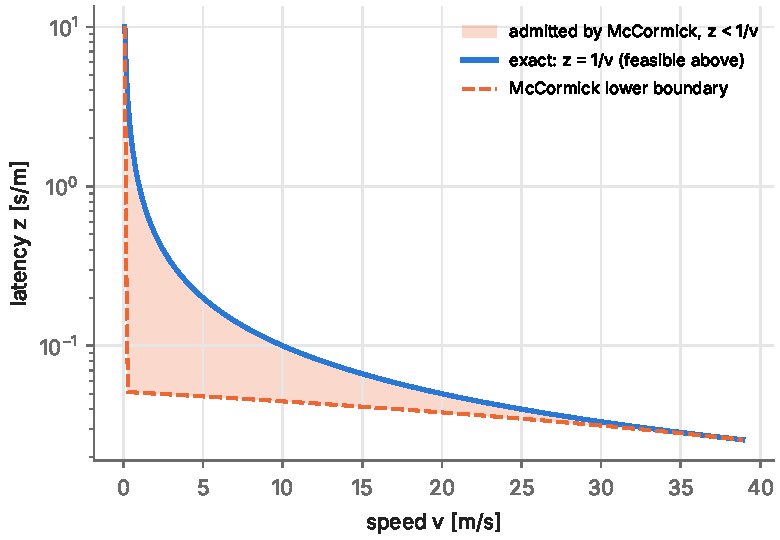
\includegraphics[width=0.62\textwidth]{../figures/mccormick_latency.pdf}
  \caption{The exact latency set $\{z \ge 1/v\}$ (above the blue hyperbola) and the set admitted by the McCormick
    envelope of $v z \ge 1$ on Example~1's box (above the dashed line). Every point in the shaded region books less
    time than the train needs.}
  \label{fig:mccormick}
\end{figure}

A solver exploits this immediately. \Cref{tab:pitfall} compares both versions on Example~1: the McCormick version
``saves'' \SI{40}{\percent} of the energy, but driving its speed profile takes \SI{674}{s} instead of \SI{540}{s}. The
point is general: McCormick envelopes are a tool \emph{inside} the branch-and-bound, where they are refined by
branching; in the model itself they change the problem.

\begin{table}[h]
\centering
\caption{Example~1 with the exact latency constraint and with its McCormick envelope (SCIP, gap \SI{0.1}{\percent}).
  The true time is recomputed from the speed profile.}\label{tab:pitfall}
\begin{tabular}{lrrrr}
\toprule
latency constraint & energy [kWh] & booked $t_N$ [s] & $\sum_k \Delta s_k / v_k$ [s] & $\min_k v_k z_k$ \\
\midrule
exact, $v_k z_k \ge 1$ & 133.0 & 540 & 540.0 & 1.000 \\
McCormick envelope & 81.1 & 540 & 674.2 & 0.048 \\
\bottomrule
\end{tabular}

\end{table}

\section{Indirect method: Pontryagin's principle}\label{sec:indirect}

\subsection{Necessary conditions}

Following \citet{Albrecht2016a} we work per unit mass: $u = F/m$, $r(v) = R(v)/m$ and the gradient acceleration
$\gamma(s) = -g\sin\alpha(s)$, so that $v\,dv/ds = u - r(v) + \gamma$. The control is bounded by
$U_-(v) \le u \le U_+(v)$ with $U_+(v) = \min(F_{\max}, P_{\max}/v)/m$ and $U_-(v) = \max(F_{\min}, P_{\min}/v)/m$.
The Hamiltonian, to be maximised, is
\begin{equation}
  H = -u^+ + \frac{\mu_1}{v} + \frac{\mu_2}{v}\big(u - r(v) + \gamma\big),
\end{equation}
with the time costate $\mu_1$ (constant, since $H$ does not depend on $t$) and the speed costate $\mu_2$. Maximising
$H$ over $u$ gives five modes in terms of the \emph{modified adjoint} $\eta = \mu_2/v - 1$:
\begin{center}
\begin{tabular}{lll}
\toprule
$\eta > 0$ & maximum power & $u = U_+(v)$ \\
$\eta = 0$ on an interval & hold at speed $V$ (HoldP) & $u = r(V) - \gamma$ \\
$-1 < \eta < 0$ & coast & $u = 0$ \\
$\eta = -1$ & switch to braking & \\
$\eta < -1$ & maximum braking & $u = U_-(v)$ \\
\bottomrule
\end{tabular}
\end{center}
Holding a speed on an interval requires $\mu_2 = v$ constant, which forces $\psi(V) + \mu_1 = 0$ with
\begin{equation}
  \psi(v) = v^2 r'(v), \qquad \varphi(v) = v\, r(v).
\end{equation}
Since $\psi$ is strictly increasing, the \emph{optimal driving speed} $V$ is determined by the time costate:
$\mu_1 = -\psi(V)$.

\paragraph{The adjoint along a phase.} On a segment with constant gradient, $\eta$ is a function of the speed only. With
$\mathcal{E}_V'(v) = (\psi(v) - \psi(V))/v^2$, which for the quadratic Davis resistance integrates to
\begin{equation}
  \mathcal{E}_V(v) = r_1 v + r_2 v^2 + \frac{\psi(V)}{v} \qquad (r(v) = r_0 + r_1 v + r_2 v^2),
\end{equation}
one finds on level track \citep[Sec.~3.5]{Albrecht2016a}
\begin{equation}\label{eq:eta}
  \eta(v) = \frac{\mathcal{E}_V(v) - \mathcal{E}_V(V)}{U_+(v) - r(v)} \ \ \text{(maximum power)}, \qquad
  \eta(v) = \frac{\mathcal{E}_V(v) - \mathcal{E}_V(V)}{-r(v)} \ \ \text{(coast)}.
\end{equation}
Both vanish at $v = V$: maximum power ends exactly when the train reaches $V$, and coasting starts from $V$.

\subsection{The braking speed as a tangent}

Coasting ends, and maximum braking begins, at the speed $U$ where $\eta(U) = -1$. By \eqref{eq:eta},
$\mathcal{E}_V(U) - \mathcal{E}_V(V) = r(U)$. Multiplying by $U$ and inserting $\psi(V)/V = r_1 V + 2 r_2 V^2$,
\begin{equation}
  \psi(V) = U\,(r_0 + 2 r_1 V + 3 r_2 V^2) = U\,\varphi'(V)
  \quad\Longrightarrow\quad
  U = \frac{\psi(V)}{\varphi'(V)} = V - \frac{\varphi(V)}{\varphi'(V)},
\end{equation}
where the last step uses $\psi = v\varphi' - \varphi$. Geometrically (\cref{fig:tangent}), \emph{$U$ is the point where
the tangent to the convex curve $\varphi(v) = v\,r(v)$ at the driving speed $V$ crosses the $v$-axis}: one Newton step
from $V$ towards the root of $\varphi$. The faster the train cruises, the earlier (at higher speed) it must start to
brake.

\begin{figure}[t]
  \centering
  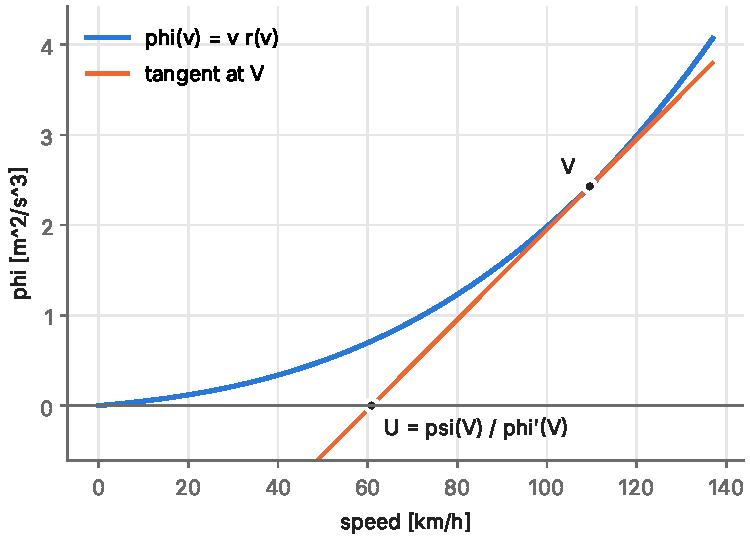
\includegraphics[width=0.48\textwidth]{../figures/brake_speed_tangent.pdf}\hfill
  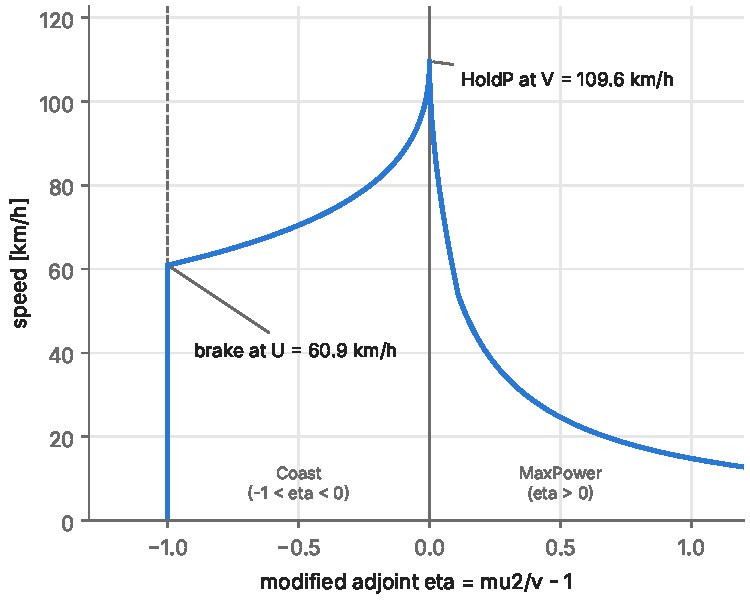
\includegraphics[width=0.48\textwidth]{../figures/phase_portrait.pdf}
  \caption{Left: the brake speed $U$ is the $v$-intercept of the tangent to $\varphi(v) = v\,r(v)$ at $V$. Right: the
    modified adjoint $\eta$ along the optimal journey on level track ($T = \SI{600}{s}$): maximum power ($\eta > 0$)
    ends at $V$, coasting runs from $\eta = 0$ to $\eta = -1$, and braking follows at $\eta = -1$
    (cf.\ Fig.~5 of \citealp{Albrecht2016a}).}
  \label{fig:tangent}
\end{figure}

\subsection{Algorithm}

On level track every phase is an explicit integral in $v$, for instance the length and duration of the
maximum-power phase,
\begin{equation}
  x_{\text{power}} = \int_0^V \frac{v\,dv}{U_+(v) - r(v)}, \qquad t_{\text{power}} = \int_0^V \frac{dv}{U_+(v) - r(v)},
\end{equation}
and similarly for coasting ($r(v)$ in the denominator) and braking ($r(v) - U_-(v)$). The hold phase closes the
distance, and an outer root search on $V$ meets the trip time (\cref{alg:indirect}). If the route is too short for a
hold phase, maximum power switches directly to coasting at some $V' < V$, and $U$ follows from $\eta(U) = -1$ on the
coasting curve that starts at $(V', 0)$. One journey takes a few milliseconds.

\begin{algorithm}[h]
\caption{Optimal journey on level track (no speed limit active, no regenerative braking)}\label{alg:indirect}
\begin{algorithmic}[1]
\Function{Journey}{$V$}
  \State $U \gets \psi(V)/\varphi'(V)$ \Comment{brake speed}
  \State compute $(x, t)$ of maximum power $0 \to V$, coasting $V \to U$, braking $U \to 0$
  \State $x_{\text{hold}} \gets S - x_{\text{power}} - x_{\text{coast}} - x_{\text{brake}}$
  \If{$x_{\text{hold}} < 0$} find $V' < V$ that closes the distance without a hold phase \EndIf
  \State \Return total time $t(V)$ and energy
\EndFunction
\State find $V$ with $t(V) = T$ by Brent's method \Comment{$t(V)$ is decreasing}
\end{algorithmic}
\end{algorithm}

\paragraph{The price of time.} The time costate has a direct economic meaning: on level track,
$-dJ^*/dT = m\,\psi(V)$, the marginal energy saved per second of additional running time. For $T = \SI{600}{s}$ a
central difference of the indirect solution gives \SI{1216.76}{kJ/s} and $m\psi(V) = \SI{1216.76}{kJ/s}$. This price
reappears in the terminal cost of the online controller \citep{RepoMPC}.

\section{Results}\label{sec:results}

\subsection{Example~1: global optimum}

Gurobi solves $\NLP$ for Example~1 ($N = 520$: ten segments of \SI{1}{m} at each end, 500 of \SI{30}{m}) to a gap of
\SI{\exGap}{\percent} in \SI{\exRuntime}{s}; SCIP needs \SI{475}{s} for a gap of \SI{0.008}{\percent}. The global
optimum uses \SI{\exEnergy}{kWh} (\SI{\exEnergyMJ}{MJ}). The relaxation is tight, $\max_k (z_k - 1/v_k) < 10^{-10}$, the dynamics residual is below $10^{-6}$, and the running time recomputed from the speed profile equals the
booked \SI{540}{s}.

\begin{figure}[t]
  \centering
  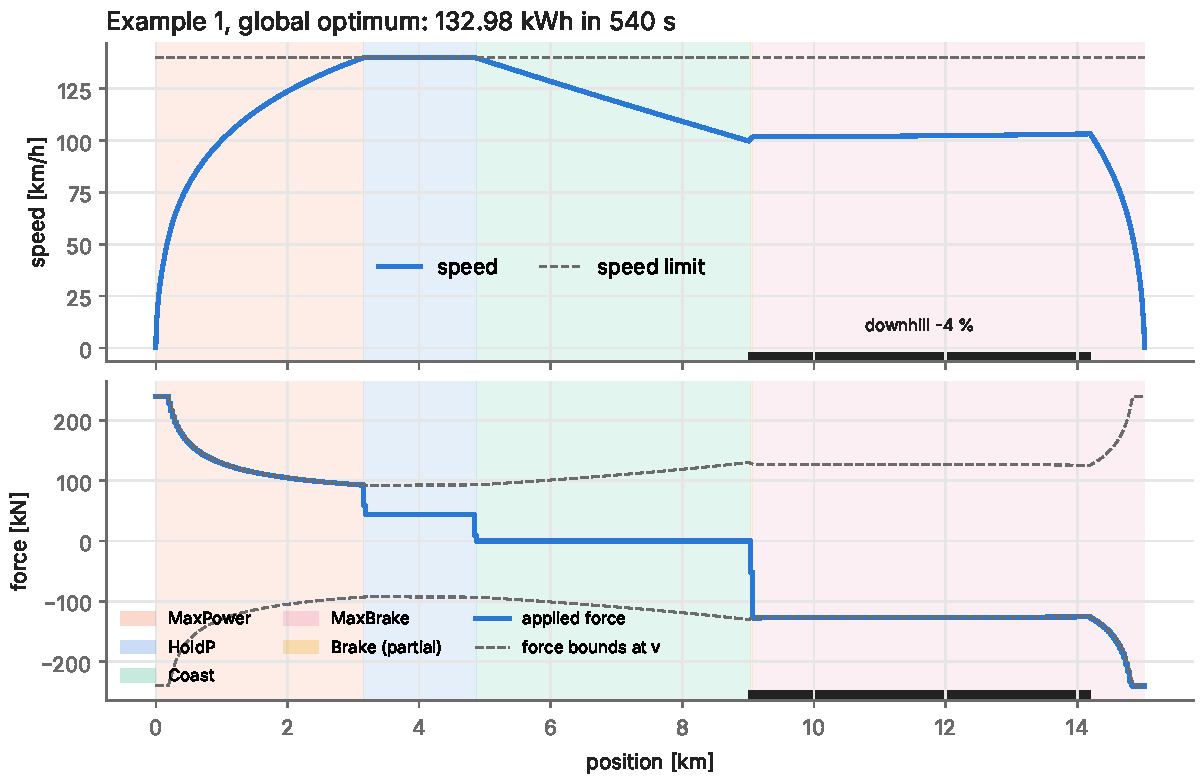
\includegraphics[width=\textwidth]{../figures/example1.pdf}
  \caption{Globally optimal speed and force profiles for Example~1, with the driving modes shaded and the
    \SI{4}{\percent} downhill section marked.}
  \label{fig:example1}
\end{figure}

The optimal strategy (\cref{fig:example1}) is maximum power up to the speed limit, holding \SI{140}{km/h}, a long
coasting phase from \SI{4.9}{km}, and \emph{maximum braking along the entire downhill section}. The reason is
physical: on a \SI{4}{\percent} gradient the gravity component is $m g \sin\alpha = \SI{156.9}{kN}$, while the braking
force is limited by the braking power to $\SI{3.6}{MW}/v$. The brakes and the running resistance can hold the speed
only if $P_{\max}/v + R(v) \ge m g \sin\alpha$, i.e.\ up to \SI{101.3}{km/h}. The train must therefore enter the
downhill section slowly enough, which is why it starts coasting more than \SI{4}{km} earlier. The planned time of
\SI{540}{s} is close to the minimum running time of the discrete model (about \SI{525}{s}), so the speed limit is
active as well; the level-track theory of \cref{sec:indirect} does not cover this case.

\subsection{Direct versus indirect method}

To compare the two methods under the assumptions of \cref{sec:indirect}, we remove the downhill section and set
$T = \SI{600}{s}$, so that the speed limit is not active. $\NLP$ is solved on meshes of \SIlist{30;15;7.5}{m}; the
indirect solution is continuous. \Cref{tab:compare} and \cref{fig:compare} show that both methods produce the same
trajectory: switching points and speeds coincide, and the energies agree to within \SI{0.07}{\percent}. The column
$T_{\mathrm{phys}}$ is explained in \cref{sec:bookkeeping}.

\begin{table}[h]
\centering
\caption{Level track, $T = \SI{600}{s}$ booked. NLP: global optimum (Gurobi). Indirect: \cref{alg:indirect} for the
  physical trip time $T_{\mathrm{phys}}$ of the NLP solution.}\label{tab:compare}
\begin{tabular}{rrrrrrr}
\toprule
$N$ & $\Delta s$ [m] & NLP$_{R3}$ [kWh] & gap [\%] & $T_\mathrm{phys}$ [s] & indirect [kWh] & diff. [\%] \\
\midrule
520 & 30 & 135.052 & 0.005 & 590.8 & 135.056 & -0.003 \\
1020 & 15 & 134.590 & 0.008 & 591.9 & 134.651 & -0.045 \\
2020 & 7.5 & 134.447 & 0.009 & 592.3 & 134.536 & -0.066 \\
\bottomrule
\end{tabular}

\end{table}

\begin{figure}[t]
  \centering
  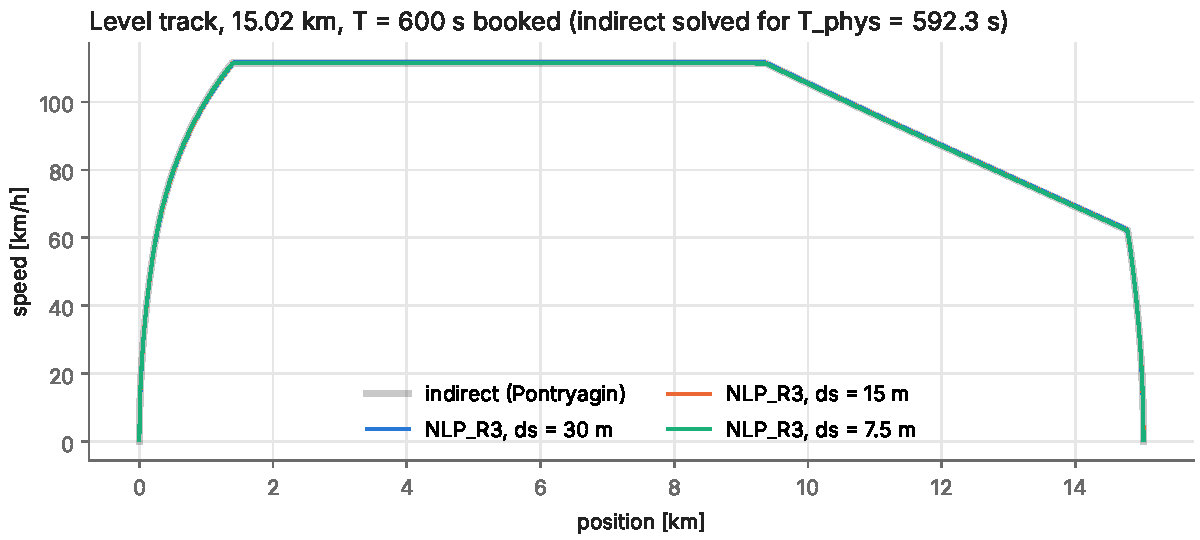
\includegraphics[width=\textwidth]{../figures/direct_vs_indirect.pdf}
  \caption{Speed profiles on level track: $\NLP$ on three meshes and the indirect solution (thick grey).}
  \label{fig:compare}
\end{figure}

Since one indirect journey costs milliseconds, the whole energy--time trade-off is available at once
(\cref{fig:energytime}). Its slope is the price of time $m\psi(V)$.

\begin{figure}[t]
  \centering
  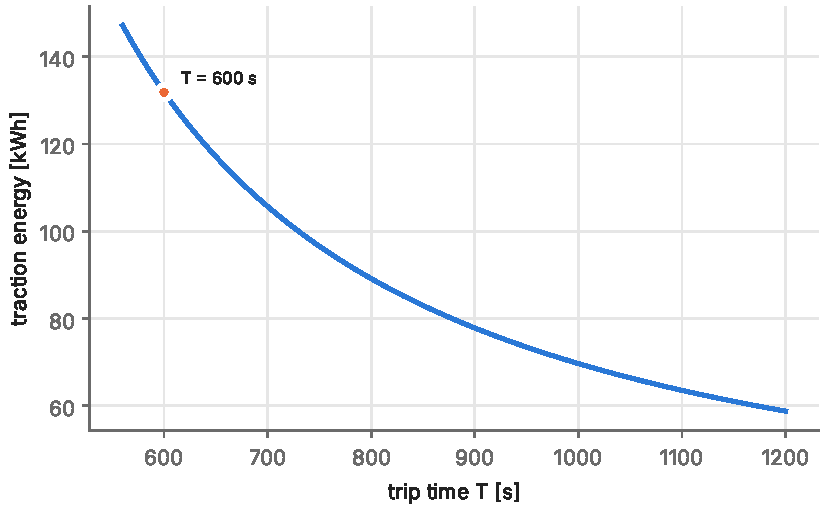
\includegraphics[width=0.6\textwidth]{../figures/energy_vs_time.pdf}
  \caption{Energy--time trade-off of the optimal journey on level track (indirect method).}
  \label{fig:energytime}
\end{figure}

\subsection{Time bookkeeping at the ends of the trip}\label{sec:bookkeeping}

The implicit scheme \eqref{eq:nlp-time} charges $t_k - t_{k-1} = \Delta s_k / v_k$ with the speed at the \emph{end} of
the segment. On the last segment $v_N = \varepsilon = \SI{0.1}{m/s}$, so the last metre costs \SI{10}{s}, whereas a
train braking through it from $v_{N-1} \approx \SI{1.09}{m/s}$ needs $2\Delta s_N / (v_{N-1} + v_N) \approx
\SI{1.65}{s}$. On the first segment the error has the opposite sign but is smaller (\SI{0.92}{s} instead of
\SI{1.69}{s}). Recomputing the time with the trapezoidal rule $\sum_k 2\Delta s_k / (v_{k-1} + v_k)$, which is exact for
constant acceleration, gives $T_{\mathrm{phys}} = \SI{530.8}{s}$ for the optimum of Example~1: the discrete model has
about \SI{9}{s} less physical driving time than $T$. The \SI{1}{m} segments at both ends, used by \citet{Xiao2025},
keep this error small, but it does not vanish under mesh refinement (\cref{tab:compare}). For the comparison with the
indirect method, and for the reference trajectory of the online controller, the booked time is therefore chosen such
that $T_{\mathrm{phys}}$ equals the planned time ($T = \SI{549.22}{s}$ for a physical \SI{540}{s} in Example~1).

\section{Conclusions and outlook}

The formulation $\NLP$ of \citet{Xiao2025} delivers certified global optima of the train eco-driving problem in seconds,
and on level track it reproduces the classical Pontryagin solution to within the discretisation error. The two
approaches complement each other: the direct method handles speed limits, steep gradients and power limits without
any case analysis, while the indirect method explains the structure of the solution --- the braking speed as a tangent
intercept, the price of time as $m\psi(V)$ --- and computes the energy--time trade-off almost for free.

Open points:
\begin{itemize}
  \item the indirect method on steep track and with speed limits (the Energymiser algorithm and the local energy
        minimisation principle of \citealp{Albrecht2016b}), which would cover Example~1 itself;
  \item regenerative braking, where hold phases at a second speed $W = \psi^{-1}(\psi(V)/\rho)$ appear;
  \item a time discretisation without the end-of-trip bias of \cref{sec:bookkeeping};
  \item time windows and fleets of trains under a green-wave policy \citep[Secs.~4--5]{Xiao2025}.
\end{itemize}

\paragraph{Acknowledgements.} I thank Sönke Lück for his guidance during the project.

\bibliographystyle{plainnat}
\bibliography{references}

\end{document}
